% !TeX program = xelatex
% !TeX encoding = UTF-8
% !TeX TXS-program:compile = txs:///xelatex | txs:///xelatex
\documentclass[aspectratio=169, table, 12pt]{beamer}
% Preamble bersama seluruh slide mata kuliah ini.
% Dipanggil dari slides/sessionXX/sessionXX.tex tepat sesudah baris
% \documentclass[aspectratio=169, table, 12pt]{beamer}
% Paket tambahan yang hanya dibutuhkan satu sesi ditulis di berkas sesi itu.

\usepackage{colortbl}
\usepackage{xcolor}
\usepackage{listings}
\usepackage{tabularx}
\usepackage{booktabs}
\usepackage{tikz}
\usepackage{pgfplots}
\pgfplotsset{compat=1.18}
\usetikzlibrary{arrows.meta, positioning, calc, fit, shapes.geometric,
	shapes.multipart, backgrounds, matrix, chains, trees}

\makeatletter
\def\input@path{{../theme/}}
\makeatother
\graphicspath{{../theme/}{../../figures/}}
\usetheme{Pradita}

\definecolor{praditagreen}{RGB}{37, 113, 71}

% Tema membuat garis tabel berwarna putih. Dikembalikan agar tabel terbaca.
\arrayrulecolor{black}
\setlength{\arrayrulewidth}{0.5pt}

\lstdefinelanguage{yaml}{
	basicstyle=\ttfamily\scriptsize,
	keywordstyle=\color{blue}\bfseries,
	commentstyle=\color{gray}\itshape,
	stringstyle=\color{red},
	showstringspaces=false,
	breaklines=true,
	frame=lines,
	numbers=none,
	backgroundcolor=\color{lightgray!10},
	tabsize=2,
	morecomment=[l]{\#}
}

\lstdefinelanguage{json}{
	basicstyle=\ttfamily\scriptsize,
	stringstyle=\color{red},
	commentstyle=\color{gray},
	breaklines=true,
	showstringspaces=false,
	tabsize=2,
	numbers=none,
	frame=lines,
	backgroundcolor=\color{lightgray!10},
	string=[s]{"}{"}
}

\lstdefinelanguage{bash}{
	keywords={},
	basicstyle=\ttfamily\scriptsize,
	ndkeywords={docker, kubectl, helm, curl, git, terraform},
	ndkeywordstyle=\color{purple}\bfseries,
	sensitive=true,
	commentstyle=\color{gray},
	numbers=none,
	breaklines=true,
	frame=lines,
	backgroundcolor=\color{lightgray!10},
	tabsize=2,
	comment=[l]{\#},
	showstringspaces=false
}

\lstdefinelanguage{http}{
	keywords={GET, POST, PUT, PATCH, DELETE, HEAD, OPTIONS, HTTP},
	basicstyle=\ttfamily\scriptsize,
	keywordstyle=\color{blue}\bfseries,
	sensitive=true,
	numbers=none,
	breaklines=true,
	frame=lines,
	backgroundcolor=\color{lightgray!10},
	tabsize=2,
	showstringspaces=false
}

\subtitle{IT40613 · Digital Platform \& API Economy}
\author{\textbf{Alfa Yohannis}}


\title{\Huge Orientasi: Platform,\\ \vspace{10pt} API, dan Capstone}
\date{Pertemuan 01}

\begin{document}
\frame{\titlepage}

\begin{frame}
  \frametitle{Isi Pertemuan}
  \vspace{14pt}
  \begin{columns}[t]
    \column{0.5\textwidth}
    {\small\tableofcontents[sections={1-3}]}

    \column{0.5\textwidth}
    {\small\tableofcontents[sections={4-6}]}
  \end{columns}
\end{frame}

\begin{frame}{\hfill}
  \centering
  \Huge{\textbf{Bila API sudah tersedia,\\mengapa surel dan berkas\\masih dipakai?}}
\end{frame}

\section{Tujuan dan Peta Mata Kuliah}

\begin{frame}{\hfill}
  \centering
  \Huge{\textbf{Tujuan dan\\Peta Mata Kuliah}}
\end{frame}

\begin{frame}{{\Large Tujuan Pembelajaran}}
  \vspace{10pt}
  \begin{itemize}
    \item Menjelaskan perbedaan bisnis \textit{pipeline} dan bisnis platform dengan contoh dari sektor yang dikenal.
    \item Menjelaskan cara kerja API (\textit{Application Programming Interface}) dengan bahasa sehari-hari, termasuk \textit{request}, \textit{response}, dan data JSON (\textit{JavaScript Object Notation}).
    \item Mengidentifikasi pertukaran data utama antara organisasi capstone dan pihak luarnya.
  \end{itemize}
\end{frame}

\begin{frame}{{\Large Banyak Pihak, Banyak Cara}}
  \vspace{6pt}
  \begin{itemize}
    \item Jaringan layanan kesehatan bertukar data dengan banyak pihak luar setiap hari.
    \item Caranya beragam: surel, unggah berkas di portal, dan sambungan khusus.
    \item Akibat pertama: antrean memanjang, karena petugas menunggu jawaban pihak lain.
    \item Akibat kedua: kerja ulang bertambah, karena data yang sama diketik ulang.
    \item Akibat ketiga: biaya integrasi naik, karena setiap pihak baru berarti satu sambungan baru.
  \end{itemize}
  \vspace{4pt}
  {\small Mata kuliah ini membahasnya dari dua sisi: platform sebagai model bisnis, API sebagai sarana teknis.}
\end{frame}

\begin{frame}{{\Large Empat Bagian Sejajar Empat Tonggak}}
  \centering
  \resizebox{0.9\textwidth}{!}{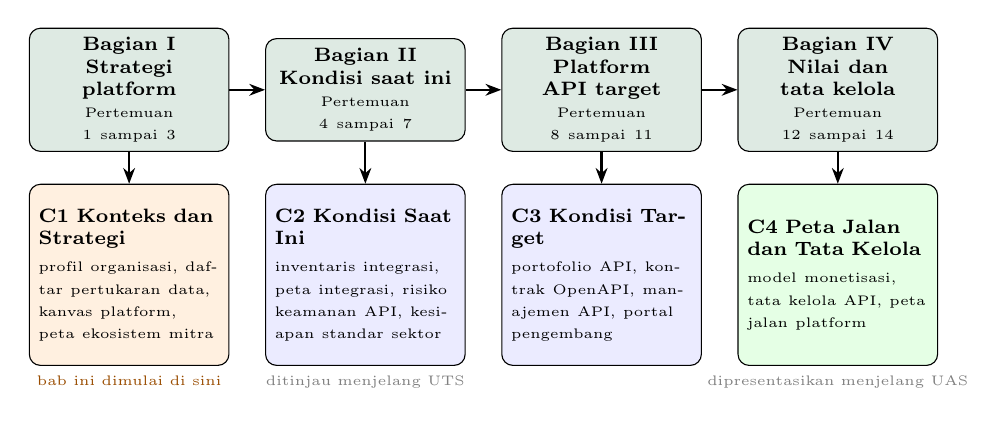
\begin{tikzpicture}[
  font=\scriptsize,
  bagian/.style={draw, rounded corners, fill=praditagreen!15, text width=2.3cm,
                 minimum height=1.3cm, align=center, font=\scriptsize\bfseries},
  tonggak/.style={draw, rounded corners, fill=blue!8, text width=2.3cm,
                  minimum height=2.3cm, align=left, font=\scriptsize},
  panah/.style={-{Stealth[length=2mm]}, thick}
]
  \node[bagian] (b1) at (0,0)
    {Bagian I\\Strategi platform\\{\tiny\mdseries Pertemuan 1 sampai 3}};
  \node[bagian] (b2) at (3,0)
    {Bagian II\\Kondisi saat ini\\{\tiny\mdseries Pertemuan 4 sampai 7}};
  \node[bagian] (b3) at (6,0)
    {Bagian III\\Platform API target\\{\tiny\mdseries Pertemuan 8 sampai 11}};
  \node[bagian] (b4) at (9,0)
    {Bagian IV\\Nilai dan tata kelola\\{\tiny\mdseries Pertemuan 12 sampai 14}};

  \node[tonggak, fill=orange!12] (c1) at (0,-2.35)
    {\textbf{C1 Konteks dan Strategi}\\[2pt]
     {\tiny profil organisasi, daftar pertukaran data, kanvas platform, peta
     ekosistem mitra}};
  \node[tonggak] (c2) at (3,-2.35)
    {\textbf{C2 Kondisi Saat Ini}\\[2pt]
     {\tiny inventaris integrasi, peta integrasi, risiko keamanan API, kesiapan
     standar sektor}};
  \node[tonggak] (c3) at (6,-2.35)
    {\textbf{C3 Kondisi Target}\\[2pt]
     {\tiny portofolio API, kontrak OpenAPI, manajemen API, portal pengembang}};
  \node[tonggak, fill=green!10] (c4) at (9,-2.35)
    {\textbf{C4 Peta Jalan dan Tata Kelola}\\[2pt]
     {\tiny model monetisasi, tata kelola API, peta jalan platform}};

  \draw[panah] (b1) -- (b2);
  \draw[panah] (b2) -- (b3);
  \draw[panah] (b3) -- (b4);
  \foreach \nomor in {1,2,3,4} {
    \draw[panah] (b\nomor) -- (c\nomor);
  }

  \node[font=\tiny, orange!60!black, anchor=north] at (c1.south)
    {bab ini dimulai di sini};
  \node[font=\tiny, gray, anchor=north] at (c2.south)
    {ditinjau menjelang UTS};
  \node[font=\tiny, gray, anchor=north] at (c4.south)
    {dipresentasikan menjelang UAS};
\end{tikzpicture}
}

  \vspace{4pt}
  {\footnotesize 14 pertemuan. Strategi dibahas lebih dahulu, karena API yang dibuka tanpa strategi hanya menambah integrasi baru yang mahal. UTS: Ujian Tengah Semester. UAS: Ujian Akhir Semester.\par}
\end{frame}

\begin{frame}{{\Large Sumbangan Empat Mata Kuliah}}
  \footnotesize
  \begin{tabularx}{\textwidth}{>{\raggedright\arraybackslash}p{5.0cm}
      >{\raggedright\arraybackslash}X}
    \hline
    \textbf{Mata kuliah} & \textbf{Sumbangan ke cetak biru} \\ \hline
    IT40513 Enterprise Architecture \& Digital Blueprint & Gambaran utuh organisasi: \textit{capability map}, \textit{value stream}, arsitektur aplikasi, dan peta jalan transformasi \\ \hline
    IT40613 Digital Platform \& API Economy & Strategi platform, potret integrasi dan API, rancangan platform API target, serta tata kelola dan peta jalan platform \\ \hline
    IT40713 Cloud-Native \& Microservices Architecture & Layanan, \textit{container}, dan infrastruktur \textit{cloud} yang menjalankan API \\ \hline
    IT40813 IT Governance, Risk \& Compliance & Kerangka risiko, keamanan informasi, dan kepatuhan \\ \hline
  \end{tabularx}

  \vspace{8pt}
  \small Tiap tim menyusun satu dokumen ``Cetak Biru Transformasi Digital'' untuk satu organisasi.
\end{frame}

\begin{frame}{{\Large Tim Campuran dan Kasus Cadangan}}
  \begin{itemize}
    \item Anggota non-teknis memimpin bagian orang, proses, dan aturan.
    \item Anggota teknis memimpin bagian sistem dan data.
    \item Tatap muka hanya hari Sabtu, untuk membahas progres capstone.
    \item Slide dipakai untuk mengulang, bukan sebagai pengganti modul.
  \end{itemize}
  \vspace{4pt}
  \begin{block}{Kasus Medikara Health}
    \small
    Tim dianjurkan memakai organisasi nyata, dengan izin tertulis dan data yang dianonimkan. Tim tanpa akses memakai Medikara Health, kasus fiktif bersama keempat mata kuliah.
  \end{block}
\end{frame}

\section{Bisnis Pipeline dan Platform}

\begin{frame}{\hfill}
  \centering
  \Huge{\textbf{Bisnis Pipeline dan\\Bisnis Platform}}
\end{frame}

\begin{frame}{{\Large Dua Cara Menciptakan Nilai}}
  \vspace{6pt}
  \begin{itemize}
    \item Bisnis \textit{pipeline} membeli bahan, mengolahnya, lalu menjual. Nilai mengalir satu arah.
    \item Bisnis platform mempertemukan produsen dan konsumen dari luar, lalu memfasilitasi interaksinya.
    \item Hagiu dan Wright, syarat pertama: interaksi langsung antara dua sisi atau lebih yang berbeda.
    \item Syarat kedua: tiap sisi bergabung atas kemauannya sendiri.
  \end{itemize}
  \vspace{4pt}
  {\small Analogi: warung makan memasak sendiri. Pujasera menyediakan tempat, kasir bersama, dan aturan.}
\end{frame}

\begin{frame}{{\Large Pola Pipeline dan Pola Platform}}
  \centering
  \resizebox{!}{0.64\textheight}{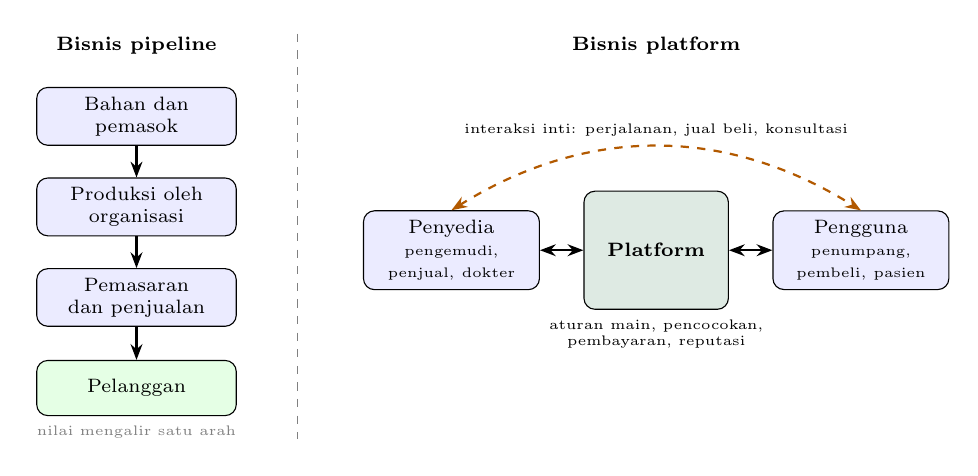
\begin{tikzpicture}[
  font=\scriptsize,
  kotak/.style={draw, rounded corners, text width=2.3cm, minimum height=0.7cm,
                align=center, font=\scriptsize},
  panah/.style={-{Stealth[length=2mm]}, thick},
  duaarah/.style={{Stealth[length=2mm]}-{Stealth[length=2mm]}, thick}
]
  % Bisnis pipeline: nilai mengalir satu arah di dalam satu organisasi.
  \node[font=\scriptsize\bfseries] at (0,2.6) {Bisnis pipeline};
  \node[kotak, fill=blue!8] (p1) at (0,1.7) {Bahan dan pemasok};
  \node[kotak, fill=blue!8] (p2) at (0,0.55) {Produksi oleh organisasi};
  \node[kotak, fill=blue!8] (p3) at (0,-0.6) {Pemasaran dan penjualan};
  \node[kotak, fill=green!10] (p4) at (0,-1.75) {Pelanggan};
  \draw[panah] (p1) -- (p2);
  \draw[panah] (p2) -- (p3);
  \draw[panah] (p3) -- (p4);
  \node[font=\tiny, gray, anchor=north] at (p4.south) {nilai mengalir satu arah};

  \draw[gray, dashed] (2.05,2.75) -- (2.05,-2.4);

  % Bisnis platform: pihak luar dipertemukan, platform mengatur interaksinya.
  \node[font=\scriptsize\bfseries] at (6.6,2.6) {Bisnis platform};
  \node[kotak, fill=blue!8, text width=2.0cm] (penyedia) at (4.0,0)
    {Penyedia\\{\tiny pengemudi, penjual, dokter}};
  \node[kotak, fill=praditagreen!15, text width=1.6cm, minimum height=1.5cm,
        font=\scriptsize\bfseries] (hub) at (6.6,0) {Platform};
  \node[kotak, fill=blue!8, text width=2.0cm] (pengguna) at (9.2,0)
    {Pengguna\\{\tiny penumpang, pembeli, pasien}};
  \draw[duaarah] (penyedia) -- (hub);
  \draw[duaarah] (hub) -- (pengguna);
  \draw[duaarah, dashed, orange!70!black] (penyedia.north) to[bend left=32]
    node[midway, above, font=\tiny, text=black]
    {interaksi inti: perjalanan, jual beli, konsultasi} (pengguna.north);
  \node[font=\tiny, align=center, anchor=north] at (hub.south)
    {aturan main, pencocokan,\\pembayaran, reputasi};
\end{tikzpicture}
}

  \vspace{2pt}
  {\footnotesize \textit{Pipeline} mengalirkan nilai satu arah di dalam satu organisasi. Platform mengatur interaksi pihak luar.\par}
\end{frame}

\begin{frame}{{\Large Tiga Pergeseran dan Dua Contoh}}
  \begin{itemize}
    \item Dari mengendalikan sumber daya sendiri ke mengorkestrasi sumber daya pihak lain.
    \item Dari mengoptimalkan proses internal ke memfasilitasi interaksi eksternal.
    \item Dari nilai bagi pelanggan ke nilai bagi seluruh ekosistem.
    \item Misalkan rumah sakit dengan 120 dokter dan 900 pasien per hari: tumbuh dengan menambah dokter, ruang, atau jam layanan sendiri.
    \item Misalkan aplikasi dengan 3.000 dokter mandiri: tumbuh saat lebih banyak dokter mandiri bergabung.
  \end{itemize}
  \vspace{2pt}
  {\footnotesize Pergeseran menurut Van Alstyne dkk. Aset utama \textit{pipeline}: gedung, stok, tenaga kerja. Aset utama platform: jaringan pihak yang bergabung dan data interaksinya.\par}
\end{frame}

\begin{frame}{{\Large Empat Jenis Platform Sehari-hari}}
  \footnotesize
  \begin{tabularx}{\textwidth}{>{\raggedright\arraybackslash}p{2.7cm}
      >{\raggedright\arraybackslash}p{2.9cm}
      >{\raggedright\arraybackslash}p{2.7cm}
      >{\raggedright\arraybackslash}X}
    \hline
    \textbf{Jenis platform} & \textbf{Sisi yang dipertemukan} & \textbf{Interaksi inti} & \textbf{Yang diatur platform} \\ \hline
    Transportasi daring & Pengemudi dan penumpang & Perjalanan atau pengantaran & Pencocokan, tarif, pembayaran, dan penilaian \\ \hline
    \textit{Marketplace} & Penjual dan pembeli & Jual beli barang & Etalase, pembayaran, ulasan, dan penyelesaian sengketa \\ \hline
    Dompet digital & Pengguna dan pedagang & Pembayaran & Saldo, kode pembayaran, dan penyelesaian dana ke pedagang \\ \hline
    Telekonsultasi & Dokter dan pasien & Konsultasi kesehatan & Verifikasi dokter, jadwal, catatan konsultasi, dan resep \\ \hline
  \end{tabularx}
\end{frame}

\begin{frame}{{\Large Saluran, Model Bisnis, dan Keterbukaan}}
  \vspace{6pt}
  \begin{itemize}
    \item Aplikasi digital adalah saluran. Platform adalah model bisnis.
    \item Pertanyaan pemeriksa: siapa yang menciptakan sebagian besar nilai yang dinikmati pengguna?
    \item Cusumano dkk.: banyak perusahaan berhasil justru memadukan \textit{pipeline} dan platform.
    \item Benzell dkk.: perusahaan yang mengadopsi API publik tumbuh tambahan 38,7 persen dibanding perusahaan serupa.
    \item API internal tidak menunjukkan efek pertumbuhan berarti. API eksternal menaikkan risiko kebocoran data.
  \end{itemize}
\end{frame}

\begin{frame}{{\Large Rumah Sakit dan Medikara+}}
  \begin{block}{Kasus Medikara Health}
    \small
    \begin{itemize}
      \item Lima rumah sakit dan 18 klinik pratama adalah \textit{pipeline}.
      \item Medikara+ masih \textit{pipeline} digital. Misalkan memuat jadwal sekitar 640 dokter, seluruhnya di fasilitas sendiri.
      \item Yang dapat dibuka: janji temu, rujukan, hasil laboratorium, pembayaran, dan layanan perusahaan klien.
      \item Bila klinik mitra, laboratorium, apotek daring, dan asuransi bergabung, Medikara+ mulai menjadi platform.
      \item Pertanyaan manajemen berubah: aturan apa yang membuat klinik mitra mau bergabung dan pasien tetap percaya.
    \end{itemize}
  \end{block}
\end{frame}

\section{API dalam Bahasa Sehari-hari}

\begin{frame}{\hfill}
  \centering
  \Huge{\textbf{API dalam\\Bahasa Sehari-hari}}
\end{frame}

\begin{frame}{{\Large Apa Itu API}}
  \begin{itemize}
    \item API adalah cara yang disepakati bagi satu sistem untuk meminta data atau layanan dari sistem lain.
    \item Peminta perlu tahu tiga hal: apa yang boleh diminta, cara menulis permintaan, dan bentuk jawabannya.
    \item \textit{Request}: formulir, yaitu permintaan dari sistem peminta.
    \item \textit{Response}: amplop atau jawaban petugas, yaitu jawaban dari sistem penyedia.
    \item \textit{Endpoint}: jendela loket, yaitu alamat tertentu pada API untuk satu jenis permintaan.
  \end{itemize}
  \vspace{2pt}
  {\footnotesize Analogi: loket hasil laboratorium. Pasien tidak pernah masuk ke ruang arsip. Kesepakatan tentang ketiga hal itu disebut kontrak API (Bab 9).\par}
\end{frame}

\begin{frame}{{\Large Isi Request dan Response HTTP}}
  \vspace{10pt}
  \begin{itemize}
    \item Sebagian besar API di web memakai HyperText Transfer Protocol (HTTP).
    \item Metode menyatakan maksud: \texttt{GET} mengambil data, \texttt{POST} mengirim data baru.
    \item Alamat menyatakan \textit{endpoint} beserta parameternya. Header memuat keterangan tambahan.
    \item Isi memuat data yang dikirim, bila ada.
    \item \textit{Response} berisi kode status, header, dan isi yang biasanya berupa JSON.
  \end{itemize}
\end{frame}

\begin{frame}{{\Large Empat Langkah Meminta Jadwal Dokter}}
  \centering
  \resizebox{!}{0.64\textheight}{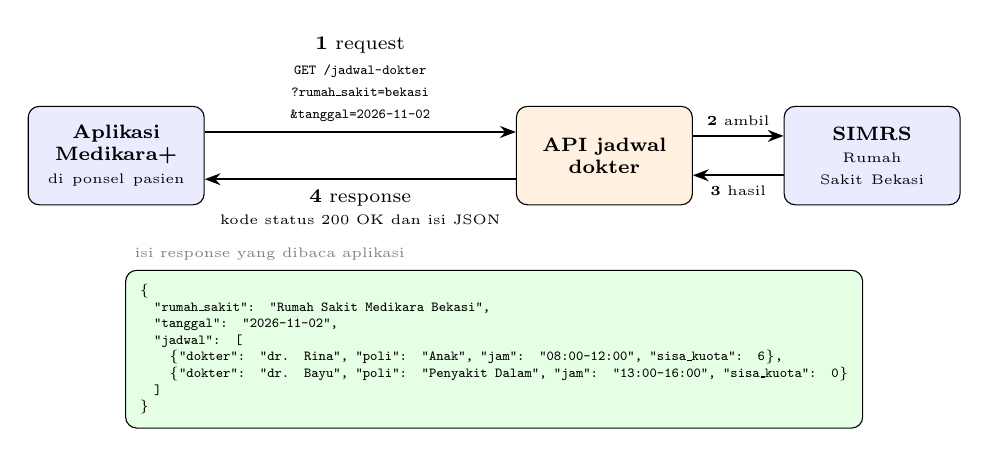
\begin{tikzpicture}[
  font=\scriptsize,
  kotak/.style={draw, rounded corners, minimum height=1.25cm, text width=2.0cm,
                align=center, font=\scriptsize\bfseries},
  panah/.style={-{Stealth[length=2mm]}, thick}
]
  \node[kotak, fill=blue!8] (aplikasi) at (0,0)
    {Aplikasi\\Medikara+\\{\tiny\mdseries di ponsel pasien}};
  \node[kotak, fill=orange!12] (api) at (6.2,0) {API jadwal\\dokter};
  \node[kotak, fill=blue!8] (simrs) at (9.6,0)
    {SIMRS\\{\tiny\mdseries Rumah Sakit Bekasi}};

  % Langkah 1 dan 4: percakapan antara aplikasi dan API.
  \draw[panah] ([yshift=0.3cm]aplikasi.east) --
    node[above, align=center, font=\scriptsize]
    {\textbf{1} request\\[1pt]
     {\ttfamily\tiny GET /jadwal-dokter}\\
     {\ttfamily\tiny ?rumah\_sakit=bekasi}\\
     {\ttfamily\tiny \&tanggal=2026-11-02}}
    ([yshift=0.3cm]api.west);
  \draw[panah] ([yshift=-0.3cm]api.west) --
    node[below, align=center, font=\scriptsize]
    {\textbf{4} response\\{\tiny kode status 200 OK dan isi JSON}}
    ([yshift=-0.3cm]aplikasi.east);

  % Langkah 2 dan 3: API mengambil data dari sistem di rumah sakit.
  \draw[panah] ([yshift=0.25cm]api.east) --
    node[above, font=\tiny] {\textbf{2} ambil} ([yshift=0.25cm]simrs.west);
  \draw[panah] ([yshift=-0.25cm]simrs.west) --
    node[below, font=\tiny] {\textbf{3} hasil} ([yshift=-0.25cm]api.east);

  % Isi response dalam format JSON.
  \node[draw, rounded corners, fill=green!10, align=left, font=\tiny\ttfamily,
        anchor=north, inner sep=5pt] (json) at (4.8,-1.45)
    {\{\\
     \quad "rumah\_sakit": "Rumah Sakit Medikara Bekasi",\\
     \quad "tanggal": "2026-11-02",\\
     \quad "jadwal": [\\
     \qquad \{"dokter": "dr. Rina", "poli": "Anak", "jam": "08:00-12:00",
       "sisa\_kuota": 6\},\\
     \qquad \{"dokter": "dr. Bayu", "poli": "Penyakit Dalam",
       "jam": "13:00-16:00", "sisa\_kuota": 0\}\\
     \quad ]\\
     \}};
  \node[font=\tiny, gray, anchor=south west] at (json.north west)
    {isi response yang dibaca aplikasi};
\end{tikzpicture}
}

  \vspace{2pt}
  {\footnotesize Vendor aplikasi tidak perlu tahu struktur basis data Sistem Informasi Manajemen Rumah Sakit (SIMRS). Rumah sakit menentukan apa yang boleh diminta: jadwal, bukan rekam medis pasien.\par}
\end{frame}

\begin{frame}{{\Large Enam Bagian JSON}}
  \footnotesize
  \begin{tabularx}{\textwidth}{>{\raggedright\arraybackslash}p{2.6cm}
      >{\raggedright\arraybackslash}p{4.2cm}
      >{\raggedright\arraybackslash}X}
    \hline
    \textbf{Bagian} & \textbf{Contoh} & \textbf{Artinya bagi pembaca} \\ \hline
    Objek & \texttt{\{ ... \}} & Satu kesatuan data, seperti satu lembar formulir \\ \hline
    Kunci dan nilai & \texttt{"poli": "Anak"} & Nama kolom dan isinya, dipisahkan titik dua \\ \hline
    Teks & \texttt{"dr. Rina"} & Isi berupa tulisan, diapit tanda petik \\ \hline
    Angka & \texttt{6} & Isi yang dapat dihitung, ditulis tanpa tanda petik \\ \hline
    Daftar & \texttt{[ \{...\}, \{...\} ]} & Beberapa isi sejenis, seperti baris-baris pada tabel \\ \hline
    Nilai khusus & \texttt{true}, \texttt{false}, \texttt{null} & Ya, tidak, dan kosong \\ \hline
  \end{tabularx}

  \vspace{6pt}
  \small Angka \texttt{6} dan teks \texttt{"6"} terlihat sama bagi manusia, tetapi berbeda bagi mesin. Jenis data setiap kunci adalah bagian dari kontrak API.
\end{frame}

\begin{frame}{{\Large Kode Status HTTP}}
  \scriptsize
  \begin{tabularx}{\textwidth}{>{\raggedright\arraybackslash}p{0.8cm}
      >{\raggedright\arraybackslash}p{3.1cm}
      >{\raggedright\arraybackslash}X
      >{\raggedright\arraybackslash}p{2.1cm}}
    \hline
    \textbf{Kode} & \textbf{Nama} & \textbf{Contoh pada jadwal dokter} & \textbf{Yang bertindak} \\ \hline
    200 & OK & Jadwal ditemukan dan dikirim & Tidak ada \\ \hline
    400 & Bad Request & Tanggal ditulis ``2 Nov'', padahal kontrak meminta \texttt{2026-11-02} & Vendor aplikasi \\ \hline
    401 & Unauthorized & Aplikasi tidak membawa identitas yang sah, misalnya \textit{token} kedaluwarsa & Vendor aplikasi \\ \hline
    403 & Forbidden & Aplikasi dikenali, tetapi meminta data yang bukan haknya & Vendor aplikasi \\ \hline
    404 & Not Found & Rumah sakit yang diminta tidak ada & Vendor aplikasi \\ \hline
    500 & Internal Server Error & SIMRS mengalami galat saat menyusun jadwal & Tim SIMRS \\ \hline
    503 & Service Unavailable & SIMRS sedang dalam pemeliharaan malam & Tim SIMRS \\ \hline
  \end{tabularx}

  \vspace{5pt}
  \footnotesize 2xx berhasil, 4xx salah pada \textit{request} peminta, 5xx masalah pada sistem penyedia. Kode 401: identitas belum terbukti. Kode 403: identitas terbukti, tetapi tidak berhak.
\end{frame}

\begin{frame}{{\Large API Bukan Akses ke Basis Data}}
  \vspace{10pt}
  \begin{itemize}
    \item Vendor dengan akun basis data dapat membaca seluruh tabel, termasuk yang tidak dibutuhkannya.
    \item Vendor dengan API hanya menerima data yang disepakati di kontrak.
    \item Akses langsung lebih cepat dibangun, tetapi perubahan struktur tabel langsung memutus aplikasi vendor.
    \item Akses langsung jauh lebih sulit diawasi: yang tercatat hanya bahwa vendor membaca tabel.
    \item Tidak tercatat data pasien mana yang dibaca dan untuk keperluan apa.
  \end{itemize}
\end{frame}

\begin{frame}{{\Large Medikara+ Meminta Jadwal Dokter}}
  \begin{block}{Kasus Medikara Health}
    \small
    \begin{itemize}
      \item Medikara+ menampilkan jadwal dari lima SIMRS yang versinya berbeda.
      \item Dua rumah sakit memakai API bawaan SIMRS. Tiga rumah sakit memberi akun yang membaca basis data setiap lima menit.
      \item Misalkan sepanjang 2025 terjadi tujuh pembaruan SIMRS. Tiap kali, jadwal kosong selama satu sampai dua hari.
      \item Pasien yang tidak menemukan jadwal datang langsung ke loket, sehingga antrean bertambah.
      \item Dengan kontrak \textit{endpoint} yang sama, pembaruan tidak lagi memutus aplikasi selama bentuk jawabannya dijaga.
    \end{itemize}
  \end{block}
\end{frame}

\section{Cara Organisasi Bertukar Data}

\begin{frame}{\hfill}
  \centering
  \Huge{\textbf{Cara Organisasi\\Bertukar Data}}
\end{frame}

\begin{frame}{{\Large Empat Cara Bertukar Data}}
  \scriptsize
  \begin{tabularx}{\textwidth}{>{\raggedright\arraybackslash}p{1.6cm}
      >{\raggedright\arraybackslash}X
      >{\raggedright\arraybackslash}X
      >{\raggedright\arraybackslash}X}
    \hline
    \textbf{Cara} & \textbf{Contoh} & \textbf{Kelebihan} & \textbf{Risiko} \\ \hline
    Manual & Surel, telepon, atau pesan singkat berisi data & Tanpa biaya awal, mudah dipahami semua pihak & Lambat, mudah salah ketik, data pribadi beredar di kotak surat \\ \hline
    Unggah berkas & \textit{Spreadsheet} atau CSV (\textit{Comma-Separated Values}) yang dikirim berkala & Sekali kirim berisi banyak baris, alatnya sudah dikenal & Format berubah tanpa pemberitahuan, kesalahan baru diketahui setelah diproses \\ \hline
    Portal web & Petugas mengetik atau mengunggah data di situs milik mitra & Mitra mengendalikan format dan pemeriksaan isian & Petugas mengetik ulang data yang sudah ada di sistem sendiri \\ \hline
    API & Sistem memanggil sistem lain secara langsung & Cepat, otomatis, kesalahan langsung terlihat lewat kode status & Biaya awal lebih tinggi, butuh kemampuan teknis, akses terlalu luas berbahaya \\ \hline
  \end{tabularx}
\end{frame}

\begin{frame}{{\Large Memilih Cara dan Membaca Survei}}
  \begin{itemize}
    \item Tidak ada cara yang selalu paling tepat. Kesalahan yang sering terjadi: memilih karena kebiasaan.
    \item Unggah berkas bulanan masuk akal untuk rekap yang jarang berubah dan dibaca manusia.
    \item API masuk akal ketika data dibutuhkan saat itu juga, misalnya status kepesertaan pasien di loket.
    \item Survei Postman 2025 (lebih dari 5.700 responden): 82 persen organisasi menerapkan \textit{API-first} pada tingkat tertentu, hanya 25 persen sepenuhnya.
    \item 65 persen memperoleh pendapatan dari API. Respondennya dekat dengan dunia API, sehingga angkanya perlu dibaca hati-hati.
  \end{itemize}
\end{frame}

\begin{frame}{{\Large Integrasi Point-to-Point dan Gejalanya}}
  \begin{itemize}
    \item Setiap pasangan sistem disambung langsung, dengan cara khusus. Bila semua saling terhubung: $n(n-1)/2$ sambungan.
    \item Enam sistem 15 sambungan, sepuluh sistem 45, dua puluh sistem 190.
    \item Gejala pertama: tidak ada orang yang memegang daftar lengkap sambungan.
    \item Gejala kedua: perubahan kecil memutus sambungan, dan baru diketahui dari keluhan pengguna.
    \item Gejala ketiga: setiap mitra baru butuh proyek integrasi baru. Gejala keempat: data yang sama berbeda isi di beberapa sistem.
  \end{itemize}
\end{frame}

\begin{frame}{{\Large Lima SIMRS: 20 Sambungan atau 9 Sambungan}}
  \centering
  \resizebox{!}{0.66\textheight}{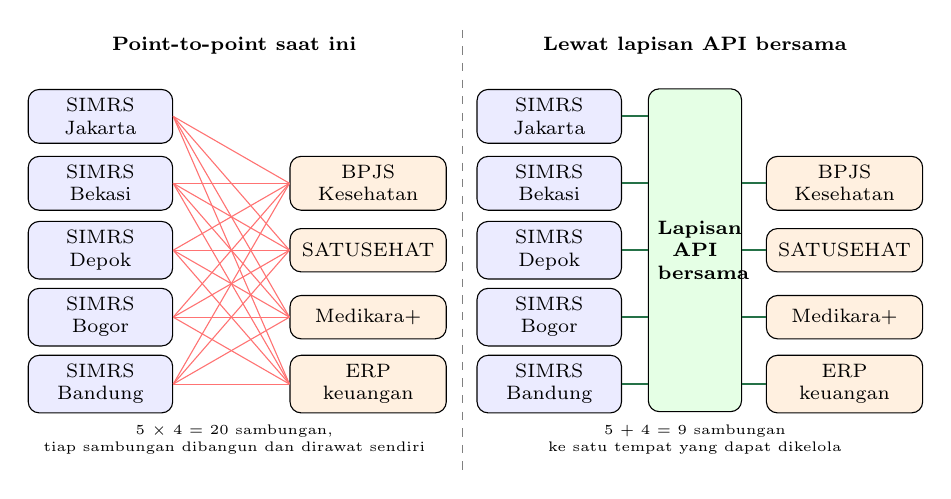
\begin{tikzpicture}[
  font=\scriptsize,
  sistem/.style={draw, rounded corners, fill=blue!8, text width=1.6cm,
                 minimum height=0.55cm, align=center, font=\scriptsize},
  tujuan/.style={draw, rounded corners, fill=orange!12, text width=1.75cm,
                 minimum height=0.55cm, align=center, font=\scriptsize},
  panah/.style={-{Stealth[length=2mm]}, thick}
]
  % Kiri: setiap SIMRS disambung langsung ke setiap tujuan.
  \node[font=\scriptsize\bfseries] at (1.7,2.65) {Point-to-point saat ini};
  \foreach \nama [count=\nomor] in {Jakarta, Bekasi, Depok, Bogor, Bandung} {
    \node[sistem] (a\nomor) at (0,{2.6-\nomor*0.85}) {SIMRS \nama};
  }
  \foreach \nama [count=\nomor] in {BPJS Kesehatan, SATUSEHAT, Medikara+,
                                    ERP keuangan} {
    \node[tujuan] (t\nomor) at (3.4,{1.75-\nomor*0.85}) {\nama};
  }
  \foreach \asal in {1,...,5} {
    \foreach \tuju in {1,...,4} {
      \draw[red!55] (a\asal.east) -- (t\tuju.west);
    }
  }
  \node[font=\tiny, align=center, anchor=north] at (1.7,-2.05)
    {5 $\times$ 4 = 20 sambungan,\\tiap sambungan dibangun dan dirawat sendiri};

  \draw[gray, dashed] (4.6,2.85) -- (4.6,-2.75);

  % Kanan: setiap sistem cukup tersambung ke satu lapisan bersama.
  \node[font=\scriptsize\bfseries] at (7.55,2.65) {Lewat lapisan API bersama};
  \foreach \nama [count=\nomor] in {Jakarta, Bekasi, Depok, Bogor, Bandung} {
    \node[sistem] (b\nomor) at (5.7,{2.6-\nomor*0.85}) {SIMRS \nama};
  }
  \node[draw, rounded corners, fill=green!10, text width=0.95cm,
        minimum height=4.1cm, align=center, font=\scriptsize\bfseries]
    (lapisan) at (7.55,0.05) {Lapisan API bersama};
  \foreach \nama [count=\nomor] in {BPJS Kesehatan, SATUSEHAT, Medikara+,
                                    ERP keuangan} {
    \node[tujuan] (u\nomor) at (9.45,{1.75-\nomor*0.85}) {\nama};
  }
  \foreach \asal in {1,...,5} {
    \draw[praditagreen, thick] (b\asal.east) -- (b\asal.east -| lapisan.west);
  }
  \foreach \tuju in {1,...,4} {
    \draw[praditagreen, thick] (u\tuju.west -| lapisan.east) -- (u\tuju.west);
  }
  \node[font=\tiny, align=center, anchor=north] at (7.55,-2.05)
    {5 + 4 = 9 sambungan\\ke satu tempat yang dapat dikelola};
\end{tikzpicture}
}

  \vspace{2pt}
  {\footnotesize Lapisan API bersama adalah gambaran awal kondisi target, bukan rancangan. ERP: \textit{Enterprise Resource Planning}.\par}
\end{frame}

\begin{frame}{{\Large Laporan Spreadsheet dan Sambungan Terpisah}}
  \begin{block}{Kasus Medikara Health}
    \small
    \begin{itemize}
      \item Setiap minggu 18 klinik pratama mengirim rekap \textit{spreadsheet} lewat surel: 936 berkas setahun.
      \item Dua staf menghabiskan sekitar tiga hari kerja per bulan. Laporan selesai sekitar tanggal 12 bulan berikutnya.
      \item Ada 10 integrasi terpisah ke Badan Penyelenggara Jaminan Sosial (BPJS) Kesehatan dan SATUSEHAT.
      \item Misalkan Rp45 juta per integrasi per tahun: sekitar Rp450 juta per tahun.
      \item Permenkes 24/2022 mewajibkan rekam medis elektronik. Yang dapat dipilih Medikara adalah cara menyambungnya.
    \end{itemize}
  \end{block}
\end{frame}

\section{Kosakata dan Kasus Berjalan}

\begin{frame}{\hfill}
  \centering
  \Huge{\textbf{Kosakata dan\\Kasus Berjalan}}
\end{frame}

\begin{frame}{{\Large Kosakata Bersama untuk Tim Campuran}}
  \scriptsize
  \begin{tabularx}{\textwidth}{>{\raggedright\arraybackslash}p{2.5cm}
      >{\raggedright\arraybackslash}X
      >{\raggedright\arraybackslash}p{4.7cm}}
    \hline
    \textbf{Istilah (Bab)} & \textbf{Arti singkat} & \textbf{Contoh di Medikara} \\ \hline
    Sisi pasar (2) & Kelompok pihak yang dipertemukan platform & Pasien dan klinik mitra pada Medikara+ \\ \hline
    Interaksi inti (2) & Pertukaran nilai utama yang difasilitasi platform & Pemesanan janji temu \\ \hline
    Efek jaringan (2) & Nilai platform naik atau turun karena jumlah pihak yang bergabung & Makin banyak klinik mitra, makin menarik bagi pasien \\ \hline
    Ekosistem (3) & Kumpulan pihak yang saling melengkapi di sekitar platform & Rumah sakit, laboratorium, apotek, dan asuransi \\ \hline
    Mitra (3) & Pihak luar yang ikut menciptakan atau menyalurkan nilai, bukan sekadar membeli & Laboratorium mitra dan asuransi \\ \hline
    Kontrak API (9) & Kesepakatan tertulis tentang apa yang boleh diminta dan bentuk jawabannya & Aturan \textit{endpoint} jadwal dokter \\ \hline
    \textit{API gateway} (10) & Pintu masuk bersama yang memeriksa dan meneruskan setiap \textit{request} & Satu pintu bagi lima SIMRS \\ \hline
    \textit{Token} (6) & Tanda pengenal digital yang membuktikan identitas dan hak akses & Tanda pengenal aplikasi Medikara+ \\ \hline
    Versi (10) & Penanda perubahan kontrak, agar pengguna lama tidak terputus & Jadwal dokter versi 1 dan versi 2 \\ \hline
  \end{tabularx}

  \vspace{3pt}
  Integrasi adalah tujuan, API salah satu caranya. Periksa cara, frekuensi, dan pemiliknya.
\end{frame}

\begin{frame}{{\Large Pihak Luar Utama Medikara Health}}
  \centering
  \resizebox{!}{0.74\textheight}{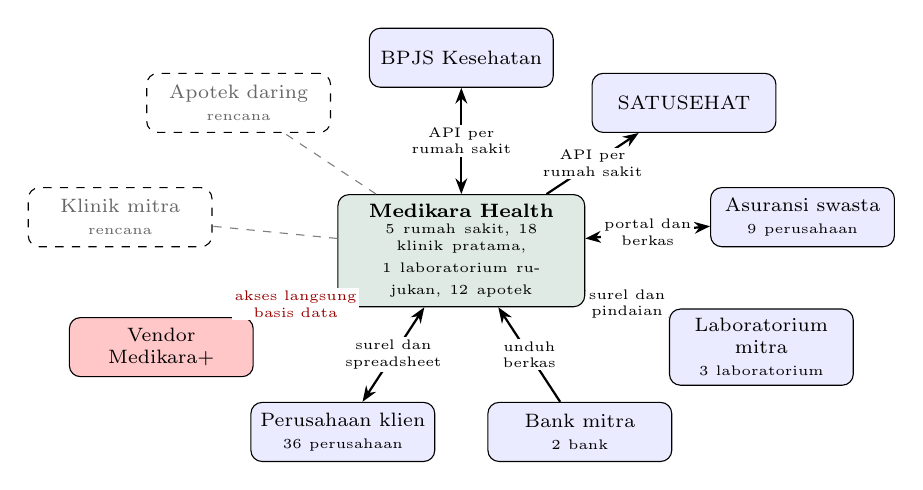
\begin{tikzpicture}[
  font=\scriptsize,
  pihak/.style={draw, rounded corners, fill=blue!8, text width=2.1cm,
                minimum height=0.75cm, align=center, font=\scriptsize},
  rencana/.style={draw, dashed, rounded corners, fill=white, text width=2.1cm,
                  minimum height=0.75cm, align=center, font=\scriptsize,
                  text=gray!80!black},
  cara/.style={midway, fill=white, font=\tiny, inner sep=1pt, align=center},
  panah/.style={-{Stealth[length=2mm]}, thick},
  duaarah/.style={{Stealth[length=2mm]}-{Stealth[length=2mm]}, thick}
]
  \node[draw, rounded corners, fill=praditagreen!15, text width=2.9cm,
        minimum height=1.3cm, align=center, font=\scriptsize\bfseries]
    (medikara) at (0,0)
    {Medikara Health\\{\tiny\mdseries 5 rumah sakit, 18 klinik pratama,\\
     1 laboratorium rujukan, 12 apotek}};

  \node[pihak] (bpjs) at (90:4.4 and 2.45) {BPJS Kesehatan};
  \node[pihak] (satusehat) at (50:4.4 and 2.45) {SATUSEHAT};
  \node[pihak] (asuransi) at (10:4.4 and 2.45) {Asuransi swasta\\{\tiny 9 perusahaan}};
  \node[pihak] (lab) at (-30:4.4 and 2.45) {Laboratorium mitra\\{\tiny 3 laboratorium}};
  \node[pihak] (bank) at (-70:4.4 and 2.45) {Bank mitra\\{\tiny 2 bank}};
  \node[pihak] (klien) at (-110:4.4 and 2.45) {Perusahaan klien\\{\tiny 36 perusahaan}};
  \node[pihak, fill=red!22] (vendor) at (-150:4.4 and 2.45) {Vendor Medikara+};
  \node[rencana] (klinik) at (170:4.4 and 2.45) {Klinik mitra\\{\tiny rencana}};
  \node[rencana] (apotek) at (130:4.4 and 2.45) {Apotek daring\\{\tiny rencana}};

  \draw[duaarah] (medikara) -- node[cara] {API per\\rumah sakit} (bpjs);
  \draw[panah] (medikara) -- node[cara] {API per\\rumah sakit} (satusehat);
  \draw[duaarah] (medikara) -- node[cara] {portal dan\\berkas} (asuransi);
  \draw[duaarah] (medikara) -- node[cara] {surel dan\\pindaian} (lab);
  \draw[panah] (bank) -- node[cara] {unduh\\berkas} (medikara);
  \draw[duaarah] (medikara) -- node[cara] {surel dan\\spreadsheet} (klien);
  \draw[duaarah, red!60!black] (medikara) -- node[cara, text=red!60!black]
    {akses langsung\\basis data} (vendor);
  \draw[gray, dashed] (medikara) -- (klinik);
  \draw[gray, dashed] (medikara) -- (apotek);
\end{tikzpicture}
}
\end{frame}

\begin{frame}{{\Large Diagram Konsep Bab 1}}
  \centering
  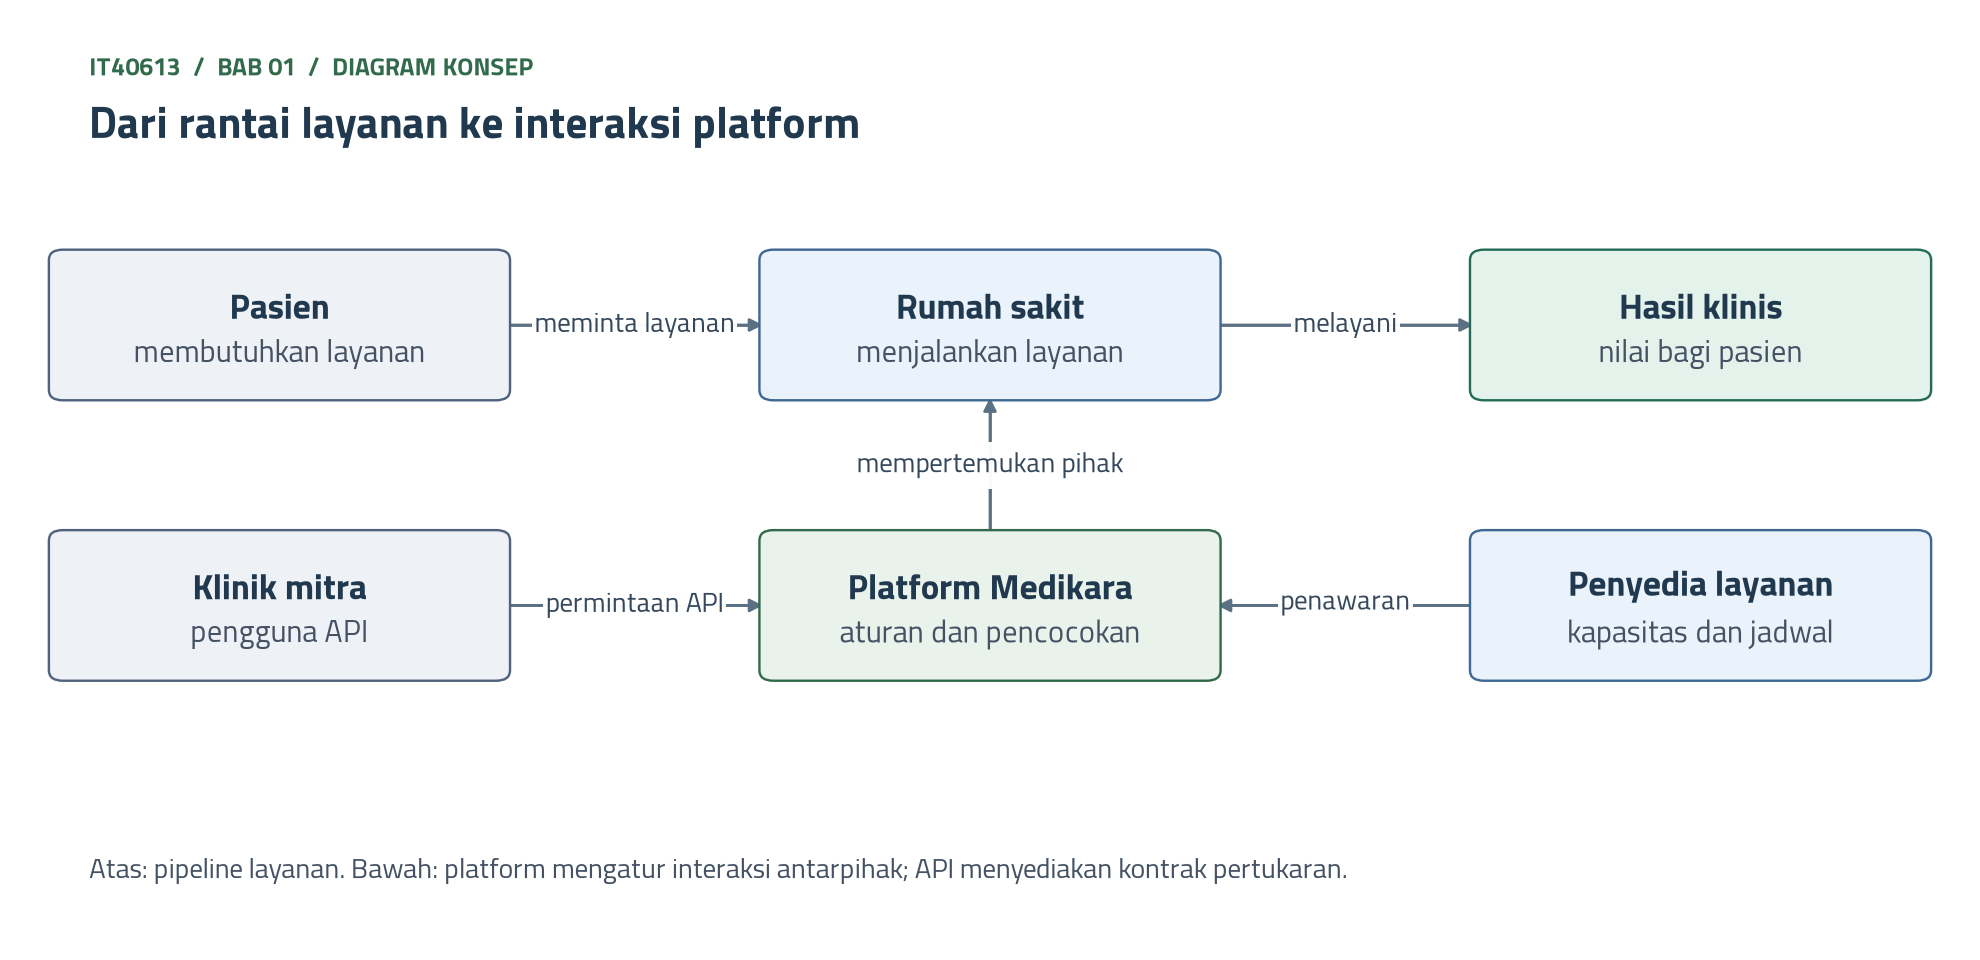
\includegraphics[width=0.96\textwidth,height=0.77\textheight,keepaspectratio]{../../figures/ch01-diagram-konsep.png}
\end{frame}

\begin{frame}{{\Large Fakta Dasar Medikara Health}}
  \scriptsize
  \begin{tabularx}{\textwidth}{>{\raggedright\arraybackslash}p{2.7cm}
      >{\raggedright\arraybackslash}X}
    \hline
    \textbf{Aspek} & \textbf{Fakta dasar} \\ \hline
    Nama & PT Medikara Nusa Sehat (``Medikara Health''), organisasi fiktif, jaringan layanan kesehatan swasta \\ \hline
    Fasilitas & 5 rumah sakit (Jakarta, Bekasi, Depok, Bogor, Bandung), 18 klinik pratama, 1 laboratorium rujukan, 12 apotek \\ \hline
    Skala & Sekitar 4.800 karyawan dan sekitar 1,2 juta kunjungan pasien per tahun \\ \hline
    Sistem saat ini & SIMRS monolitik \textit{on-premise} dengan versi berbeda karena hasil akuisisi; ERP keuangan terpusat; Medikara+ buatan vendor \\ \hline
    Integrasi dan data & \textit{Point-to-point} ke BPJS Kesehatan dan SATUSEHAT yang berbasis HL7 FHIR; data pasien tersebar; banyak laporan disusun dengan \textit{spreadsheet} \\ \hline
    Strategi 2026 sampai 2030 & ``Satu Pasien, Satu Rekam Medis'': layanan terintegrasi lintas fasilitas, ekosistem mitra, modernisasi ke \textit{cloud}, kepatuhan pada Undang-Undang Pelindungan Data Pribadi (UU PDP) dan aturan rekam medis elektronik \\ \hline
    Pemicu perubahan & Kebocoran data pasien skala kecil lewat vendor pada 2025; temuan audit tentang kontrol akses yang lemah; antrean panjang; biaya integrasi tinggi \\ \hline
  \end{tabularx}
\end{frame}

\begin{frame}{{\Large Kasus untuk Seluruh Semester}}
  \begin{block}{Kasus Medikara Health}
    \small
    \begin{itemize}
      \item Bagian I menguji apakah Medikara layak menjadi pengatur ekosistem kesehatan.
      \item Bagian II memotret integrasi \textit{point-to-point}, Medikara+, dan kebocoran lewat vendor.
      \item Bagian III memakai janji temu, hasil laboratorium, dan layanan kesehatan karyawan sebagai calon API prioritas.
      \item Bagian IV membahas harga, tata kelola mitra, persaingan usaha, dan agen AI (\textit{Artificial Intelligence}) dari perusahaan klien.
      \item Skenario pengandaian selalu ditandai dengan kata ``Misalkan''.
    \end{itemize}
  \end{block}
\end{frame}

\section{Aktivitas, Ringkasan, dan Latihan}

\begin{frame}{\hfill}
  \centering
  \Huge{\textbf{Aktivitas, Ringkasan,\\dan Latihan}}
\end{frame}

\begin{frame}{{\Large Aktivitas: Tim dan Pertukaran Data}}
  \begin{itemize}
    \item Tujuan: tim campuran terbentuk, organisasi capstone terpilih, daftar pertukaran data tersusun.
    \item Peran: koordinator, pemimpin wawancara, penelusur dokumen, pencatat cara pertukaran.
    \item Langkah: profil satu halaman, wawancara, enam sampai sepuluh pihak luar, tiga pertukaran paling bermasalah.
    \item Luaran: profil organisasi dan daftar pertukaran data, masuk ke tonggak C1 Konteks dan Strategi.
    \item Penilaian: kelengkapan 30 persen, ketepatan 25 persen, kejelasan masalah 25 persen, etika 20 persen.
  \end{itemize}
  \vspace{2pt}
  {\footnotesize Izin tertulis wajib, data dianonimkan, tanpa data pribadi pasien atau karyawan. Berkas: \berkas{sources/chapter01/}.\par}
\end{frame}

\begin{frame}{{\Large Ringkasan}}
  \vspace{6pt}
  \begin{itemize}
    \item Keragaman cara bertukar data menimbulkan antrean, kerja ulang, dan biaya integrasi yang terus naik.
    \item \textit{Pipeline} menciptakan nilai lewat rantai sendiri. Platform mempertemukan pihak luar dan mengatur interaksinya.
    \item API hanya memberikan data yang disepakati di kontrak. Kode 4xx untuk peminta, 5xx untuk penyedia.
    \item Lima SIMRS dan empat tujuan butuh 20 sambungan. Sepuluh sambungan saja memakan sekitar Rp450 juta per tahun.
    \item Platform dan API dimulai dari peta hubungan organisasi dengan pihak luarnya, bukan dari teknologi.
  \end{itemize}
\end{frame}

\begin{frame}{{\Large Latihan}}
  \vspace{6pt}
  \begin{itemize}
    \item Latihan 1, \textit{Pipeline} atau Platform: satu layanan digital diuji dengan empat pertanyaan pemeriksa.
    \item Latihan 2, Menjelaskan Jadwal Dokter kepada Rekan Non-Teknis: penjelasan tanpa singkatan, dibacakan kepada satu rekan.
    \item Latihan 3, Klaim Asuransi lewat Unggah Berkas dan lewat API: misalkan 2.400 klaim per bulan, sekitar 6 persen ditolak karena format.
  \end{itemize}
  \vspace{6pt}
  {\small Dikerjakan secara pribadi. Yang dinilai adalah penalaran dan perbandingannya. Berkas: \berkas{sources/chapter01/}.\par}
\end{frame}

\end{document}
